\section{Location Framework}
We will start a detailed discussion about the UIFramework with an in-depth look
into the structure of the AdminCentral web application and its backbone - the
\emph{Location Framework}.

As it was discussed in the beginning of the chapter AdminCentral web application
is based on Vaadin framework. According to chapter \ref{chapter_tech_stack}
Vaadin applications work on top of Java Servlet API and any logic that is
executed within application is triggered by user input within the web browser.
An application is responsible for loading, displaying and closing the proper
views on a screen in response on the various events. Typically Vaadin
application would create, attach or detach components, set up the references
between them and update the states of components.

We have stated in chapter \ref{thesis_problems} that one of the most crucial
goals of the project is to provide an extensible and highly-customizable user
interface allowing for adding and removing the functional components on demand.
This requirement implies that AdminCentral web application must obtain an
abstact framework for the state management. An obvious solution would be to
provide mappings between possible URL's and the views. Such mappings should be
easilly customizable and the views should be possible to be pre-created as well
as generated on the fly (e.g. - based on the parameters of the query). All these
statements bring us to the navigation management framework called \emph{Location
Framework}.

Navigation handling is one of the most common problems that Rich Internet
Applications (RIA) developers face. For instance - dealing with poor support of
the browsers' history. The source of the problem is the fact that the frameworks
like GWT usually provide capabilities for building the single-paged applications
with an only one highly dynamic page that generates HTML-views according to
UI-logic. In such situations teh browser is not responsible for tracking the
navigation. For instance if a user presses the "back" button he will most likely
navigate away from the application, which is usually not the desired behavior.
However, this problem is possible to handle by means of a framework. GWT, for
instance, provides the API for the interaction with a web-browser history based
on fragments.
Fragment is a part of a URL after the hash sign (\#). Changing a URL-fragment
does not trigger a browser refresh, so a framework can provide the track of an
application internal navigation history by manually pushing the items into
browser history \cite{gwt_historian}.  Let us consider an example:
\url{http://www.example.com/example_app#view1}

In this example everything before the hash sign \texttt{(\#)} is the example-app
URL and the \texttt{view1} is the identifier of some application UI state. If a
user navigates to this URL in a browser GWT will fire an internal event and the
application client-side logic will determine which user interface parts to
display.

However, URL fragment is just a tool that could be used for navigation.The main
problem is how to effectively map the multiple views that a complex Rich
Internet Application might provide to the corresponding URL fragments. It also
should be possible to serialize the state of the views in the fragment and many
others.
For native GWT applications the framework team has provided a rather flexible
and useful sub-framework called Activities and Places framework
\cite{activities_places}.

Activities and Places is a design pattern for structuring the navigation in a
user interface. The parts of an application are its activities and they can be
reached by activating their respective place. For web applications a place is
derived from the browser URL allowing a section of the application to be
bookmarked. As the user interacts with the application the browser URL changes
in response to place changes.

Activities and Places framework is widely used by the GWT community. However,
for a server-side oriented application like Magnolia 5.0 AdminCentral it would
be impossible to use it for navigation, as the client-side is rather thin. As a
consequence it was decided by the development team to port the framework to the
server-side and adopt it for Vaadin-based applications. The resulting concept is
called the Location framework. The name location was chosen to substitute the
term place because it reflects the web nature of the application better: the
current URL of a RIA or a site is obtained by calling \texttt{window.location}
in JavaScript.  Let us consider the Locations framework in details.

\subsection{Location}

\begin{figure}[H] \centering 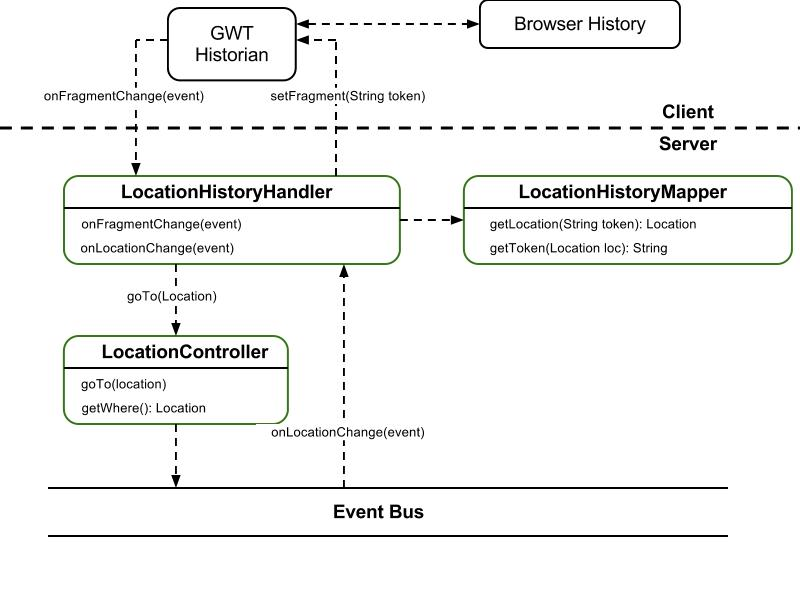
\includegraphics[width=\textwidth]{location_arch.jpg}
	\caption{Location framework pt.1}
	\label{fig:location_arch}
\end{figure}

\subsubsection{Location} 
Location is a data transfer interface between the server-side and
the browser history. It is capable of deserializing a fragment string into a 
Plain Old Java Object (POJO). That POJO in turn can serialize itself into a
valid URL fragment string.

\subsubsection{Event Bus}
 The backbone of the Location framework is the EventBus
(\emph{TODO Consider EventBus pattern appendix}). One global event bus acts as a communication
channel between other parts of the framework. For instance, it gets notified of
the fragment change from the client-side and triggers the user interface
change sequence. On the other hand, when a UI update is initiated on the
server-side due to some user input and an application navigates to a new
location, an event bus propagates the new location to all the interested
parties. The location is eventually transformed into the fragment and ends up on
the client-side in the browser history.

\subsubsection{Location Controller} \texttt{LocationController} is a singleton
(/*consider appendix*/) object that handles navigation between locations and keeps
current location. \texttt{LocationController} is tightly
connected with the event bus:
the latter accepts the listeners and transmits the events fired by the
controller. In order to perform navigation to a different location through the
\texttt{LocationController} one has to simply call the following:

\begin{lstlisting}
	locationContoller.goTo(location);
\end{lstlisting}

Such a call changes and controller's current location and causes it to emit a
LocationChangeEvent on the event bus. A good example of a
\texttt{LocationChangeEvent} handler would be some kind of a UI manager that
would find and/or construct the appropriate view depending on a location.

\subsubsection{LocationHistoryHandler and LocationHistoryMapper} 
Another entity that handles the \texttt{LocationChangeEvents} is
\texttt{LocationHistoryHandler}.
It is the connection point between the framework and the web browser. It is
capable of converting the location into a string (URL fragment) and vice-versa -
obtaining a location by a fragment. However, \texttt{LocationHistoryHandler}
does not accomplish these tasks on its own rather than that - delegating the
implementations of search and conversion to a \texttt{LocationHistoryMapper}.
\texttt{LocationHistoryMapper} as it is stated in its title maps the unique
history fragments to corresponding locations in a bi-directional way.


\subsection{Activities and ActivityManagers}
\begin{figure}[H] \centering 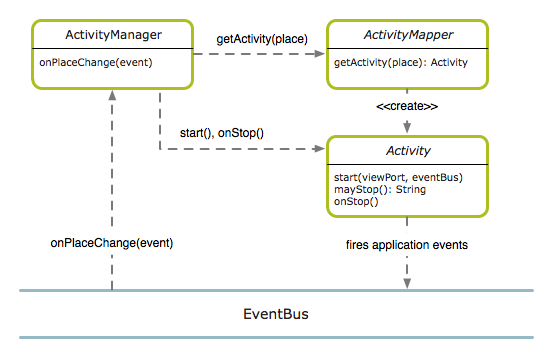
\includegraphics[width=\textwidth]{activities.png}
	\caption{Location framework pt.2}
	\label{fig:location_arch}
\end{figure}

\subsubsection{Activity}
\texttt{Activity} is the concept of the original framework from Google Web
Toolkit. Its main purpose is similar to the role of the Presenter in
Model-View-Presenter pattern which will be discussed later in the current
chapter (see \ref{MVP}). Provided with a state snapshot stored in a location and
a viewport for rendering an \texttt{Activity} is able to handle state,
initialize, update, load and unload the \texttt{View}\cite{activities_places}.
\texttt{Activity} is also able to notify the other objects (e.g. a different
\texttt{Activity}) about its internal events through the framework's
\texttt{EventBus}.
 
\subsubsection{ActivityManager and ActivityMapper}
\texttt{ActivityManager} and \texttt{ActivityMapper} classes purpose is to
resolve an
\texttt{Activity} that corresponds to an incoming \texttt{Location}.
\texttt{ActivityManager} subscribes to an \texttt{EventBus} and awaits for new
\texttt{Locations}.An \texttt{ActivityMapper} is used as a registry that mapps 
an \texttt{Activity} to a \texttt{Location}.

In Locations framework the role of the Activities is played by the
\emph{Apps} and the job of \texttt{ActivityManager}
and \texttt{ActivityMapper} is done by an \texttt{AppController} (see \ref{section_apps}).


 